\documentclass{article}
\usepackage{fullpage,amsmath,amsthm,graphicx,enumitem,amsfonts}
\usepackage{multicol}
\usepackage{booktabs}
\usepackage{algorithm}
\usepackage{algpseudocode}
\usepackage{sgame}

\usepackage{tikz}
\usetikzlibrary{positioning, shapes, arrows, fit}

\theoremstyle{definition}
\newtheorem{thm}{Theorem}
\newtheorem{question}[thm]{Question}
\newenvironment{solution}{\noindent\textit{Solution:}}{}

\title{ASEN 5264 Decision Making under Uncertainty\\
       Exam 2: POMDPs and Games}

\date{}

\begin{document}
\maketitle

\begin{question}(20 points)
    Two autonomous vehicles approach a narrow one-lane passage from opposite directions. Each vehicle must choose whether to go ($G$) or yield ($Y$).

    If both vehicles choose $G$, they block each other and both receive a payoff of $-2$.
    If one vehicle chooses $G$ and the other chooses $Y$, the vehicle that goes receives a payoff of $2$.
    Any vehicle that chooses $Y$ receives a payoff of $0$.

    This yields the following payoff matrix:
    \begin{center}
    \begin{game}{2}{2}
        & $G$ & $Y$ \\
        $G$ & $-2, -2$ & $2, 0$ \\
        $Y$ & $0, 2$ & $0, 0$
    \end{game}
    \end{center}

    \begin{enumerate}[label=\alph*)]
        \item If player 1 plays $G$, what is player 2's best response? Justify your answer.
        \item There are three Nash equilibria for this game. Describe the joint policies in all three of these equilibria. If you need to, you may express part of your answer as a set of unsolved linear equations, but clearly indicate how solving these equations yields a joint policy.
        \item Name a solution concept besides the Nash equilibrium that would yield an outcome that is better in some sense than any of the Nash equilibria. Briefly justify why this is better and explain how this could be implemented in this setting in real life.
    \end{enumerate}
\end{question}

\clearpage

\begin{question}(30 points)
    As you prepare for a dry summer, consider the following POMDP: Your friend has asked you to water her garden. The garden has two states, healthy and dry, $\underline{S=\{H,D\}}$. After work, you can either get your hose and go \underline{water} the garden, stop by and \underline{check} it on your way home, or do \underline{nothing}, $\underline{A=\{W,C,N\}}$. Each day that the garden starts out healthy (including days after you water), it has a 10\% chance of becoming dry by the next day, resulting in the following transition matrices:
    \begin{align*}
        T^W = \begin{bmatrix}
            0.9 & 0.1 \\
            0.9 & 0.1
        \end{bmatrix},
        \qquad
        T^C = \begin{bmatrix}
            0.9 & 0.1 \\
            0.0 & 1.0
        \end{bmatrix},
        \qquad
        T^N = \begin{bmatrix}
            0.9 & 0.1 \\
            0.0 & 1.0
        \end{bmatrix}.
    \end{align*}
    Taking into account your trouble and the health of the garden, you receive reward \underline{$R(s,a)$} defined in the table below:
\begin{center}
    \begin{tabular}{c|rrr}
         & $W$ & $C$ & $N$ \\
        \hline
        $H$ & $0$ & $4$ & $5$ \\
        $D$ & $0$ & $-6$ & $-5$
    \end{tabular}
\end{center}
After each action, you make an assessment (observation) of the garden's next state, \underline{$O=\{H,D\}$}. If you check, you receive a perfect observation; if you water or do nothing, you receive an uninformative observation (always $H$). This results in the following observation distribution:
\begin{align*}
    Z(o \mid a, s') = \begin{cases}
        1 & \text{if } a = C \text{ and } o = s' \\
        1 & \text{if } a \in \{W,N\} \text{ and } o = H \\
        0 & \text{otherwise}
    \end{cases}
\end{align*}
The discount factor is \underline{$\gamma = 1.0$} (we will only consider two-step horizons).
\begin{enumerate}[label=\alph*)]
    \item Consider the three following two-step conditional plans, $\pi_A$, $\pi_B$, and $\pi_C$:
    \begin{center}
    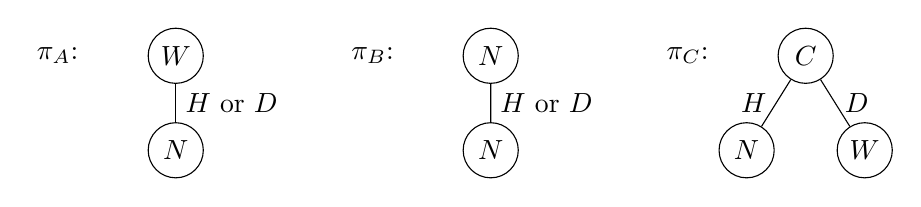
\begin{tikzpicture}[
        circlenode/.style={circle, draw, minimum size=0.7cm, inner sep=0pt},
        level distance=1.2cm, sibling distance=1.5cm,
        edge from parent/.style={draw}
    ]
    \node at (-1.5, 0) {$\pi_A$:};
    \node[circlenode] (a0) at (0,0) {$W$}
        child { node[circlenode] {$N$} edge from parent node[right] {$H$ or $D$} };
    \node at (2.5, 0) {$\pi_B$:};
    \node[circlenode] (b0) at (4,0) {$N$}
        child { node[circlenode] {$N$} edge from parent node[right] {$H$ or $D$} };
    \node at (6.5, 0) {$\pi_C$:};
    \node[circlenode] (c0) at (8,0) {$C$}
        child { node[circlenode] {$N$} edge from parent node[left] {$H$} }
        child { node[circlenode] {$W$} edge from parent node[right] {$D$} };
    \end{tikzpicture}
    \end{center}
    Compute the two-step $\alpha$-vector for $\pi_C$.
    \item The two-step $\alpha$-vectors for $\pi_A$ ($[4, 4]$) and $\pi_B$ ($[9,-10]$) are shown in a plot on the answer sheet. Draw the $\alpha$-vector for $\pi_C$ on the same plot and label it.
    \item The table below shows all but one of the two-step $Q$-values for the underlying MDP (i.e. the $Q_\text{MDP}$ values). Find the missing value, $Q_\text{MDP}(H, N)$.
        \begin{center}
            \begin{tabular}{c|rrr}
                 & $W$ & $C$ & $N$ \\
                \hline
                $H$ & $4.5$ & $8.5$ & ? \\
                $D$ & $4.5$ & $-6$ & $-5$
            \end{tabular}
        \end{center}
    \item In the plot on the answer sheet, draw the QMDP two-step pseudo-$\alpha$-vectors for each action.
    \item Briefly describe the differences between the policies defined by the QMDP two-step pseudo-$\alpha$-vectors and the two-step $\alpha$-vectors for $\pi_A$, $\pi_B$, and $\pi_C$.
\end{enumerate}

\end{question}

\clearpage


\begin{question}(10 points)
    Consider a discounted infinite-horizon two-player Markov game defined by $(I, S, A, T, R, \gamma)$ with discrete $S$ and $A$.

    \begin{enumerate}[label=\alph*)]
        \item Suppose Player 2's policy $\pi^2$ is fixed. Explain how Player 1 could calculate a best response.

        \item Suppose the players alternately replace their current policies with best responses to the other player's current policy. After $|S|$ iterations of this process, are the best response policies guaranteed to constitute a Nash equilibrium?

        \item Your friend gives you a joint policy $(\pi^1,\pi^2)$ that he claims is a Nash equilibrium, but you suspect it is not. How could you prove that his claim is false?
    \end{enumerate}
\end{question}





\end{document}
